\documentclass[a4paper]{article} %
\usepackage{graphicx,amssymb} %
%\usepackage[left=35mm, right=35mm, top=15mm, bottom=20mm, noheadfoot]{geometry}
\usepackage[utf8]{inputenc}
\usepackage{caption}
\usepackage{subcaption}
\graphicspath{{figuras/}}


\textwidth=15cm \hoffset=-1.2cm %
\textheight=25cm \voffset=-2cm %

\pagestyle{empty} %

\date{} %

%\def\keywords#1{\begin{center}{\bf Keywords}\\{#1}\end{center}} %
\def\keywords#1{{\bf Keywords: }{#1}}

% begin the document
\begin{document}
\thispagestyle{empty}

\title{\textbf{Title}}

% Authors
\author{Anderson A. Borba, \\ 
         PPGEEC - Programa de Pós-Graduação em Engenharia Elétrica e Computação\\
	 Universidade Presbiteriana Mackenzie\\
	 ISITEC - Instituto Superior de Inovação e Tecnologia\\
         São Paulo, Brasil\\ \\ % Affiliation 1
         Maurício Marengoni  \\ % If any other author with different Affilation
	 Universidade Presbiteriana Mackenzie\\
         São Paulo, Brasil \\ \\ % Affiliation 2 (if needed)
	% New author \\
	% New affiliation \\
	% Add authors and affiliation as needed
	\tt{anderborba@gmail.com} % Only one corresponding e-mail
}%

\date{} % <--- leave date empty
\maketitle\thispagestyle{empty} %% <-- you need this for the first page


\begin{abstract}
	Estudo sobre equações anisotrópicas aplicadas em imagens.
\end{abstract}

\keywords{Multigrid Methods, Computational Vision, Edge detection, Sobel operators, Laplacian methods.}

\section{Introdução}

Este artigo está baseado nas ideias proposta no artigo \cite{tsiotsios2013anisotropic}, o intuíto é investigar a resolução da equação diferencial anisotrópica e propor uma resolução mais eficiênte da mesma. 

\section{Difusão anisotrópica}


E equação da anisotropia pode ser modelada por 

\begin{equation}\label{eq2}
\left\{\begin{array}{lc}
I_t=div(c(x,y,t)\nabla I), & \forall x,y\in \Omega\\
I(x,y,t)=g, & \forall x,y\in\partial{\Omega}\\
I(x,y,t_0)=I_0(x,y,0), & \forall x,y\in \Omega
\end{array}
\right.
\end{equation}

Onde $t$ é um parametro de tempo, $I(x,y,0)$ é a imagem original e $\nabla I(x,y,t)$ é o gradiente da imagem para cada tempo $t$, e $c(x,y,t)=g(||\nabla I(x,y,t)||)$ é chama de função de condutância responsável pela anisotropia da equação diferencial.

A função $g$ é escolhida para satisfazer a difusão máxima em regiões uniformes e e que a difusão é interrompida pelas as arrestas, isto é, respectivamente respectivamente $\lim_{x\rightarrow 0}g(x)=1$ e $\lim_{x\rightarrow\infty}g(x)=0$. No artigo \cite{perona1990scale} foram propostas duas funções
\begin{equation}\label{eq3}
\begin{array}{lcl}
g_{1}(x,y,t)&=&\exp\left[-\left(\frac{x}{K}\right)^2\right]\\
\end{array}
\end{equation}

e 

\begin{equation}\label{eq4}
\begin{array}{lcl}
	g_{2}(x,y,t)&=&\frac{1}{1+\left(\frac{x}{K}\right)^2}\\
\end{array}
\end{equation}
onde $K$ é um limiar para a magnitude do gradiente que controla a razão da difusão e serve como um limiar suave entre os gradientes das imagens que são atribuídos ao ruído e aqueles atribuídos as bordas.

No artigo \cite{black1998robust} foi proposta outra função de condutância denominada função duplamente pesada de Turkey


\begin{equation}\label{eq5}
	g_{3}(x)=\left\{\begin{array}{lc}
		\frac{1}{2}\left[1-\left(\frac{x}{S}\right)^2\right]^2, & \forall x<S\\
		0, & \mbox{caso contrário}
\end{array}
\right.
\end{equation}
onde $S=\sqrt{2}K$.

Definimos a função fluxo por $\phi(x):=g(x)x$ que representa a soma do fluxo de brilho qu é gerado. O fluxo máximo é gerado nos locais onde $|\nabla I|=K$.

\subsection{Discretização da equação anisotrópica}
A discretização de equação (\ref{eq2}) pode ser representada pela equação algébrica discreta

\begin{equation}\label{eq6}
 I_{i,j}^{t+1} = a_eI_{i+1,j}^{t}+a_wI_{i-1,j}^{t}+a_cI_{i,j}^{t}+a_nI_{i,j+1}^{t}+a_sI_{i,j-1},
\end{equation}
sendo $a_e,a_w,a_c,a_n,$ e $a_s$ coeficientes da equação discreta de difusão anisotrópica. Cada um desses coeficientes dependen da posição do pixel e ainda do tempo em que são calculados.  

A equação algébrica discreta pode ser representada pela notação usando estencil ou núcleo
$$I_{i,j}^{t+1}=\left[
\begin{array}{lrl}
 0 &  a_n & 0\\
 a_w &  a_c & a_e\\
 0 &  a_s & 0\\
\end{array}
\right]_{3 \times 3}*I_{i,j}^{t}$$

\subsection{Validação e verificação da acurácia para a equação isotrópica}

Nesta seção serão definidos os problemas para a validação dos códigos implementados e sua respectivas acurácia.

Inicialmente vamos resolver a equação da difusão isotrópica
\begin{equation}
\begin{array}{lllll}
	\frac{\partial I(x,y,t)}{\partial t}&=&\nabla I(x,y,t). &(x,y)\in&D\\ 
	I(x,y,0)& = & g(x,y) & (x,y)\in & D\\
	I(x,y,t)& = & h(x,y,t) & (x,y)\in&\partial D\\
\end{array}\label{equa1:1}
\end{equation}

A discretização será realizada por diferênças finitas de primeira ordem no tempo e segunda ordem no espaço (Domínio $D$). Realizando o processo de discretização obteremos a seguinte equação algébrica:
\begin{equation}
\begin{array}{lll}
	I_{i,j}^{t+1} &=& I_{i+1,j}^{t}+I_{i-1,j}^{t}+I_{i,j}^{t}+I_{i,j+1}^{t}+I_{i,j-1}-4I_{i,j}^t,\label{equa1:2}
\end{array}\label{equa1:2}
\end{equation}

que pode ser representada pelo seguinte núcleo:
$$L I(x,y)^{t+1}=\left[
\begin{array}{lrl}
 0 &  1 & 0\\
 1 &  4 & 1\\
 0 &  1 & 0\\
\end{array}
\right]_{3 \times 3}* I(x,y)^{t},$$

A validação será testada no seguinte exemplo no qual também mostraremos a acurácia:
\begin{equation}
\begin{array}{lllll}
	\frac{\partial I(x,y,t)}{\partial t}&=&\nabla I(x,y,t). &(x,y)\in&[0,1]\times[0,1]\\ 
	I(x,y,0)& = & g(x,y) & (x,y)\in & D\\
	I(x,y,t)& = & h(x,y,t) & (x,y)\in&\partial D\\
\end{array}\label{equa1:3}
\end{equation}

onde a condição inicial é dada por,
\begin{equation}
\begin{array}{lllll}
	I(x,y,0)&=&g(x,y)& = & \exp(x+y). \\
\end{array}\label{equa1:4}
\end{equation}
onde as condições de contorno são dadas por,
\begin{equation}
\begin{array}{lllll}
	h(0,y,t)& = &\exp(y+2t),  & 0\leq t \leq T,&0\leq y \leq 1 . \\
	h(1,y,t)& = &\exp(1 + y + 2t),  & 0\leq t \leq T,&0\leq y \leq 1 . \\
	h(x,0,t)& = &\exp(x+2t),  & 0\leq t \leq T,&0\leq x \leq 1 . \\
	h(x,1,t)& = &\exp(1+x+2t),  & 0\leq t \leq T,&0\leq x \leq 1 . \\
\end{array}\label{equa1:5}
\end{equation}


No caso destes testes conhecemos a solução exata que será usada para verificar a acurácia com auxilio da norma do máximo, isto é, $erro=\Vert I-\bar{I}\Vert$, onde $I$ é a solução exata e $\bar{I}$ a solução aproximada.
\begin{equation}
\begin{array}{lll}
	I(x,y,t)& = & \exp(x+y+2t). \\
\end{array}\label{equa1:4}
\end{equation}
\begin{figure}[!htb]
\centering
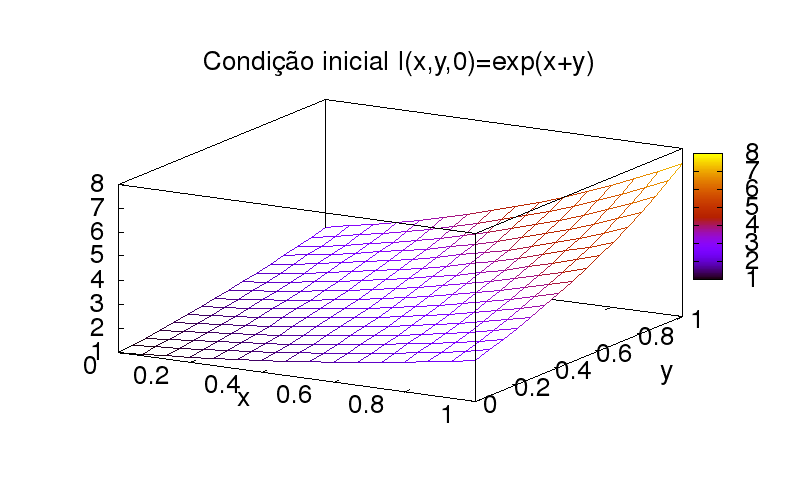
\includegraphics[width=2.5in]{cond_inic.png}
\label{fig5}
\caption{Condição inicial.}
\end{figure}

\subsubsection{Verificação da acurácia}

A tabela mostra a acurácia e a ordem de aproximação da discretização na domínio $D$.

\begin{table}[!h]
\begin{tabular}{|c|c|c|}
\hline
	n & erro& razão\\
\hline
	16 & 0.002130709465& ****\\
\hline
	32 &0.000500641341&    4.2560 \\
\hline
	64 &0.000121225177     &   4.1298  \\
\hline
128	 &   0.000029839353  &    4.0625 \\
\hline
256	 &   0.000007401560  &  4.0315   \\
\hline
\end{tabular}
\end{table}

É destacado na 3 coluna da tabela a razão entre os consecutivo erros (norma do máximo entre a solução aproximada e a solução exata no devido tempo). Esse é o comportamento esperado para o erro de uma discretização por diferenças finitas de ordem $2$ no domínio $D$, como é o caso da discretização realizada nesta pesquisa. 


\begin{figure}[!htb]
\centering
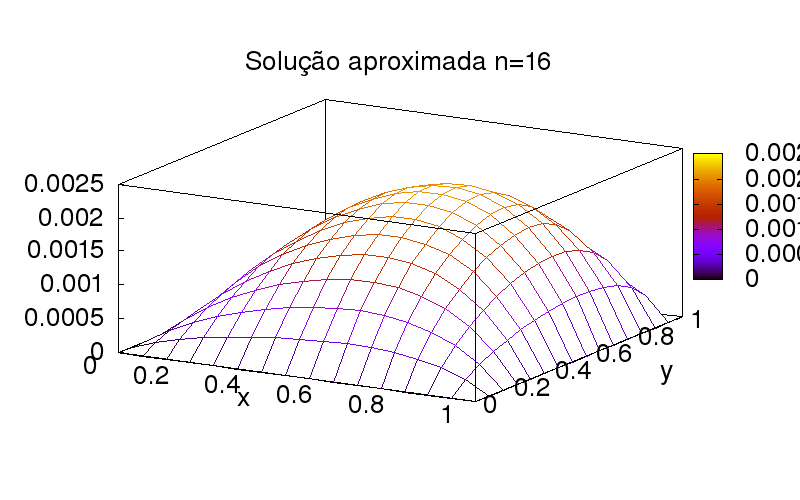
\includegraphics[width=2.5in]{erro_n_16.png}
\label{fig5}
\caption{Erro para $n=16$.}
\end{figure}

\begin{figure}[!htb]
\centering
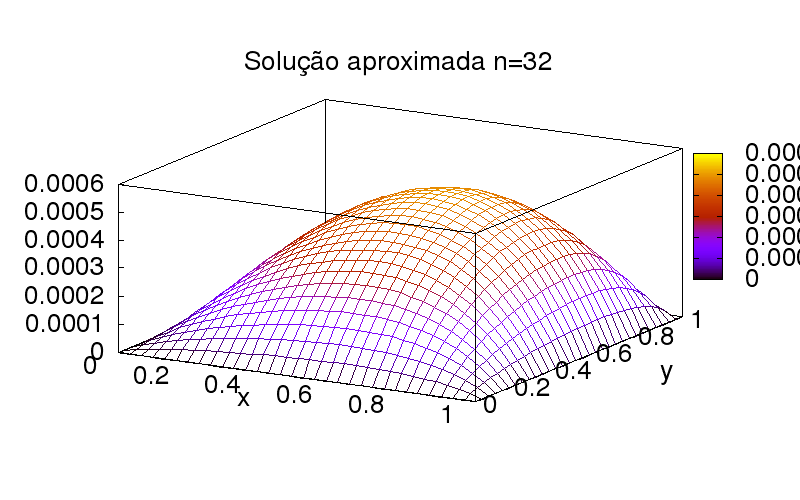
\includegraphics[width=2.5in]{erro_n_32.png}
\label{fig5}
\caption{Erro para $n=32$.}
\end{figure}
\begin{figure}[!htb]
\centering
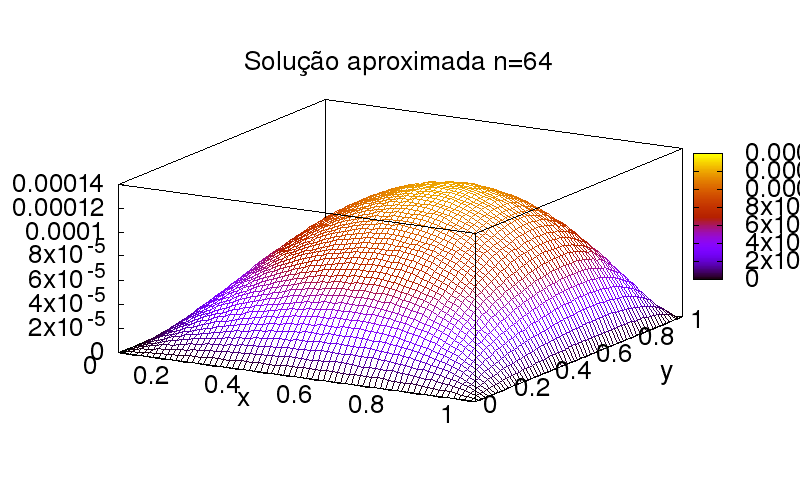
\includegraphics[width=2.5in]{erro_n_64.png}
\label{fig5}
\caption{Erro para $n=64$.}
\end{figure}
\begin{figure}[!htb]
\centering
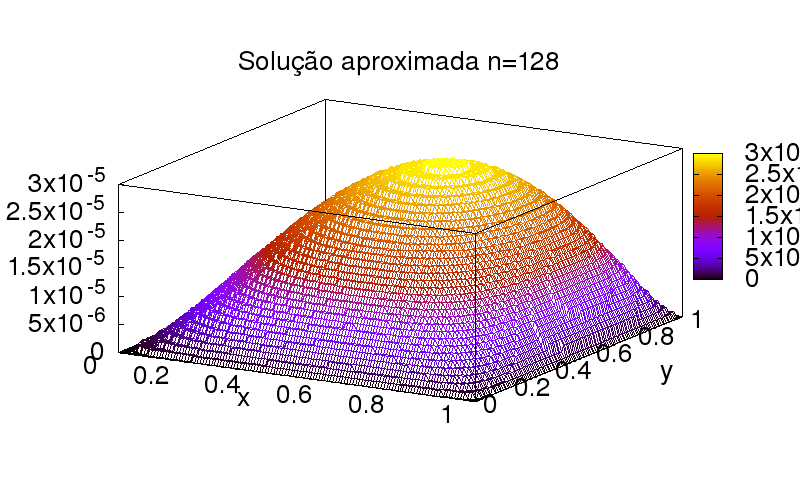
\includegraphics[width=2.5in]{erro_n_128.png}
\label{fig5}
\caption{Erro para $n=128$.}
\end{figure}

\begin{figure}[!htb]
\centering
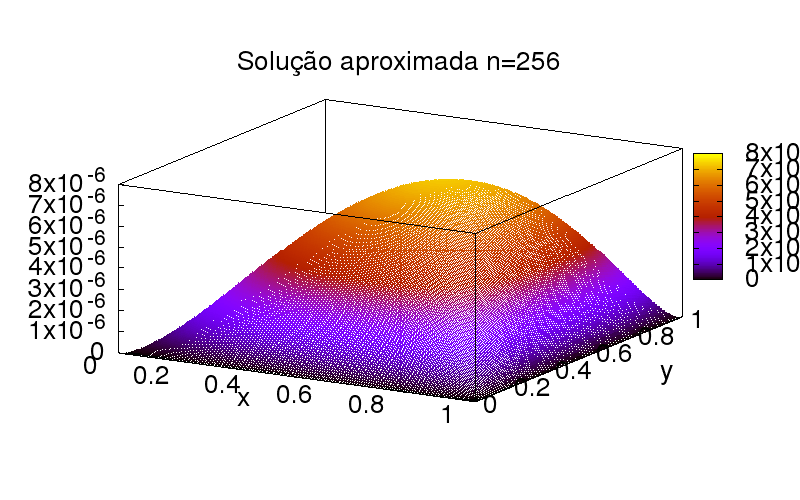
\includegraphics[width=2.5in]{erro_n_256.png}
\label{fig5}
\caption{Erro para $n=256$.}
\end{figure}

\subsection{Discretização da equação anisotrópica}

Seja a equação anisotrópica (\ref{eq2}) e seu domínio. A discretização na variável tempo será realizada da mesma maneira como na equação isotrópica, a mudança irá ocorrer na discretização da variável bidimensional no espaço, para mais detalhes pode-se ler as referências \cite{perona1990scale} e \cite{chen2011iterative}.

Discretização de primeira ordem da variável tempo
\begin{equation}\label{eq6}
\begin{array}{llll}
	I_t&=&\left.\frac{\partial I}{\partial t}\right|_{i,j}&=\frac{I_{i,j}^{t+1}-I_{i,j}^{t}}{\Delta t}.\\
\end{array}
\end{equation}

Discretização do termo advectivo anisotrópico
\begin{equation}\label{eq7}
	div(c(x,y,t)\nabla I)=div(c\nabla I)_{i,j}^{t},\\
\end{equation}
para isso, usaremos aproximações de segunda ordem do polinômio de Taylor,
\begin{equation}\label{eq8}
\begin{array}{lrl}
	div(c\nabla I)_{i,j}^{t}&=&\frac{1}{h^2}\left[c_{i+\frac{1}{2},j}I_{i+1,j}^{t}+c_{i-\frac{1}{2},j}I_{i-1,j}^{t}+c_{i,j+\frac{1}{2}}I_{i,j+1}^{t}+c_{i,j-\frac{1}{2}}I_{i,j-1}^{t}\right.\\
	&-&\left.(c_{i+\frac{1}{2},j}+c_{i-\frac{1}{2},j}+c_{i,j+\frac{1}{2}}I_{i,j+1}+c_{i,j-\frac{1}{2}})I_{i,j}^{t}\right].\\
\end{array}
\end{equation}
e realizando o algebrismo necessário na equação (\ref{eq2})

\begin{equation}\label{eq9}
	\left.\frac{\partial I}{\partial t}\right|_{i,j}^{t+1}=div(c\nabla I)_{i,j}^{t}\\
\end{equation}

\begin{equation}\label{eq10}
	\frac{I_{i,j}^{t+1}-I_{i,j}^i{t}}{\Delta t}=div(c\nabla I)_{i,j}^{t}\\
\end{equation}
\begin{equation}\label{eq11}
	I_{i,j}^{t+1}=I_{i,j}^{t}+\Delta tdiv(c\nabla I)_{i,j}^{t}\\
\end{equation}
é finalizado a discretização da mesma, tal que podemos representa-lá como a equação algébrica discreta
\begin{equation}\label{eq12}
 I_{i,j}^{t+1} = a_eI_{i+1,j}^{t}+a_wI_{i-1,j}^{t}+a_cI_{i,j}^{t}+a_nI_{i,j+1}^{t}+a_sI_{i,j-1},
\end{equation}
sendo   
\begin{equation}\label{eq13}
\begin{array}{lrl}
	a_e & = & c_{i+\frac{1}{2},j},\\
	a_w & = & c_{i-\frac{1}{2},j},\\
	a_n & = & c_{i,j+\frac{1}{2}},\\
	a_s & = & c_{i,j-\frac{1}{2}},\\
	a_c & = & 1 - \Delta_t(a_e+a_w+a_n+a_s).\\
\end{array}
\end{equation}

A equação algébrica discreta pode ser representada pela notação usando estencil ou núcleo
$$I_{i,j}^{t+1}=\left[
\begin{array}{lrl}
 0 &  a_n & 0\\
 a_w &  a_c & a_e\\
 0 &  a_s & 0\\
\end{array}
\right]_{3 \times 3}*I_{i,j}^{t}.$$

\subsubsection{Validação e verificação da acurácia para a equação anisotrópica}

Para validar e verificar a acurácia da implementação e discretização da equação de difusão anisotrópica é necessário testar nesse momento somente a discretização na variável espacial, pois o {\it setup} da evolução no tempo é o mesmo do algoritmo anterior. Para isso, usaremos o exemplo $1$ do artigo \cite{wang2005new} que trata da equação governate para estado estacionário da equação do calor em meios anisotrópicos.




\subsection{Características das funções de condutância}


%\begin{figure}[!htb]
%\minipage{0.32\textwidth}
%  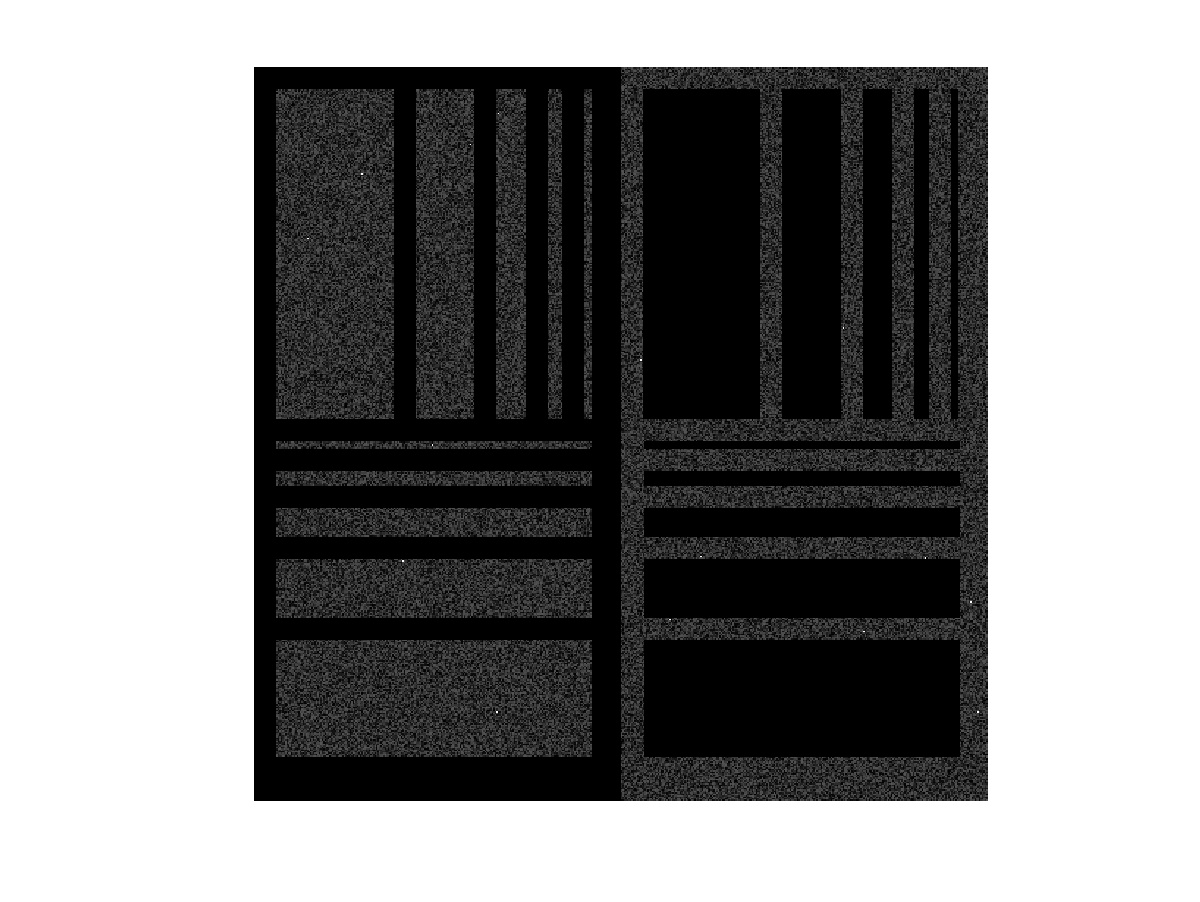
\includegraphics[width=\linewidth]{Eq_Phantom_0p000_4_1_1.jpg}
%	\caption{Phantom $P_{1,4,0.0}$}\label{fig:awesome_image1}
%\endminipage\hfill
%\minipage{0.32\textwidth}
%  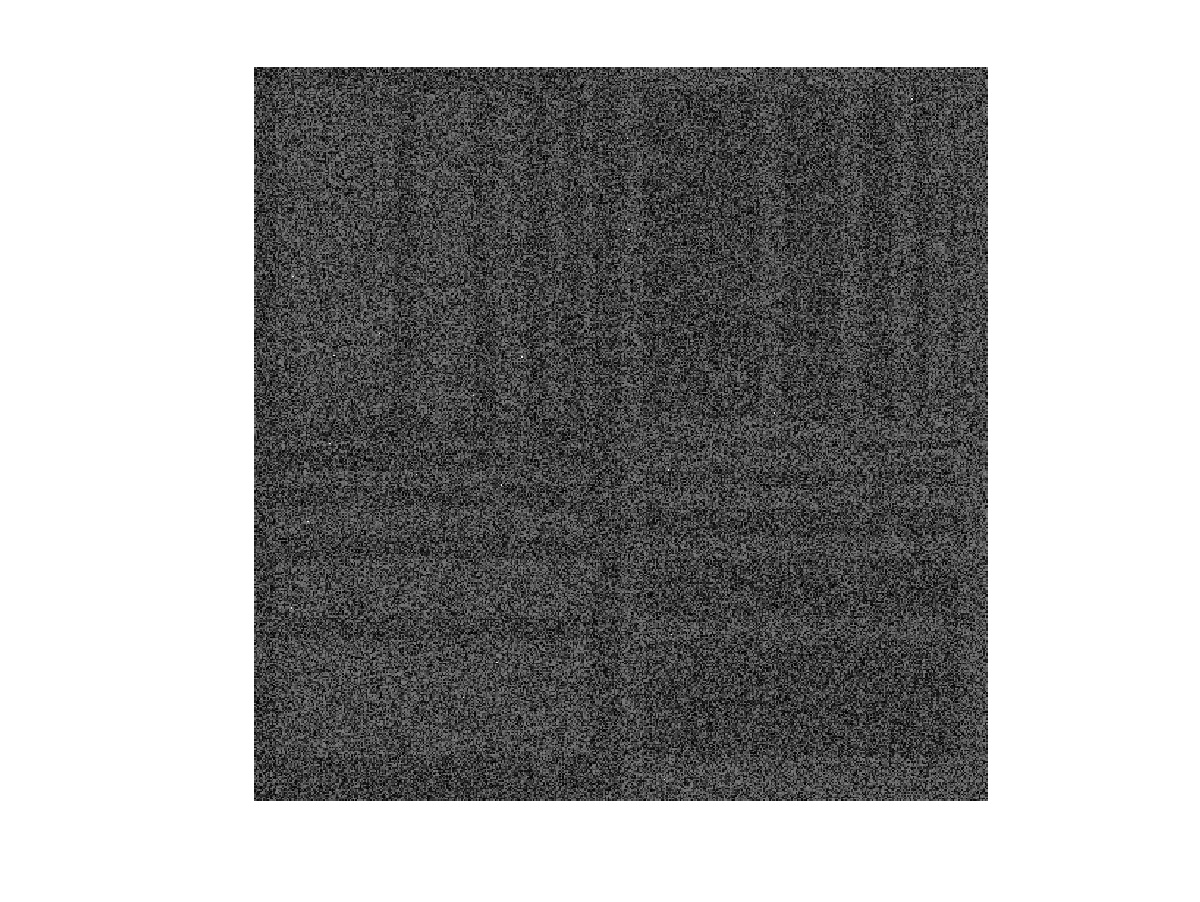
\includegraphics[width=\linewidth]{Eq_Phantom_0p500_4_1_1.jpg}
%	\caption{Phantom $P_{1,4,0.5}$}\label{fig:awesome_image1}
%\endminipage\hfill
%\minipage{0.32\textwidth}%
%  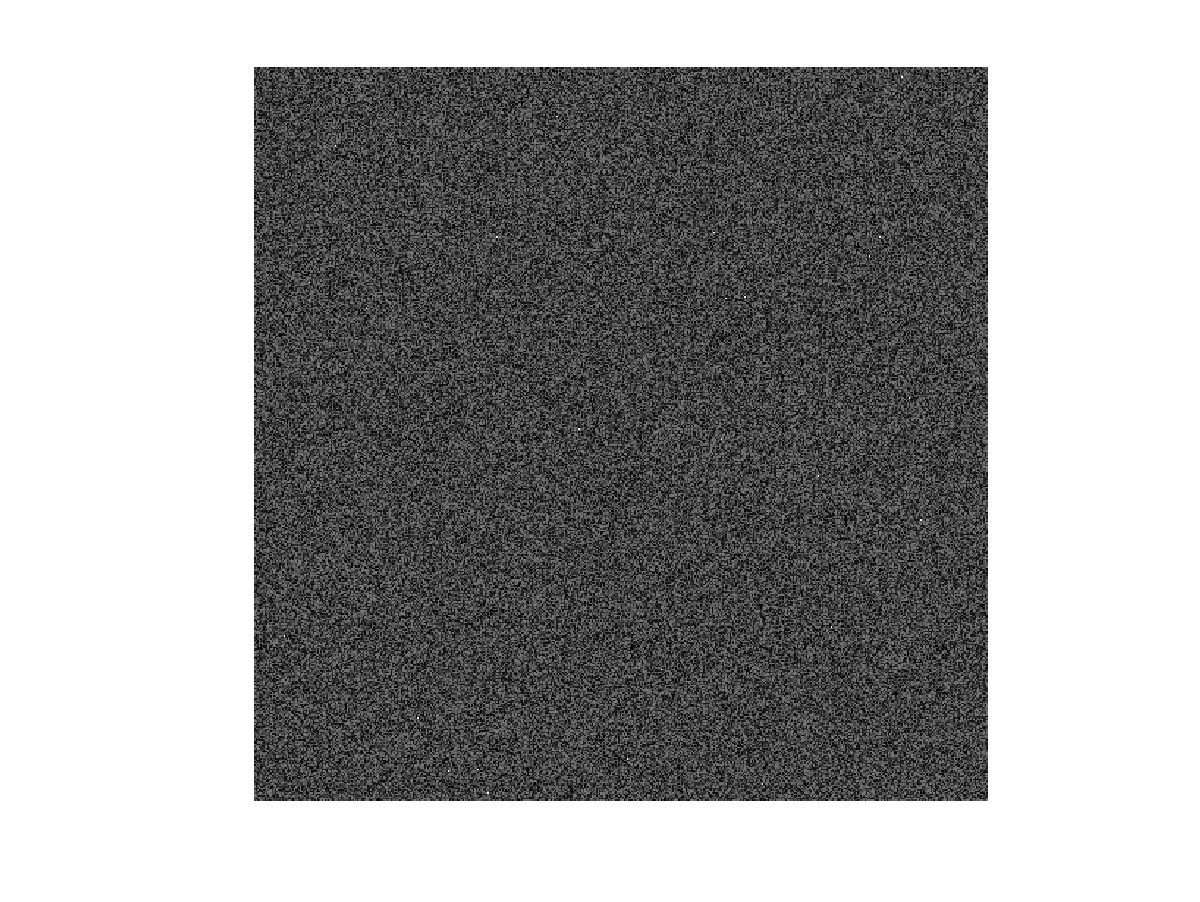
\includegraphics[width=\linewidth]{Eq_Phantom_0p700_4_1_1.jpg}
%	\caption{Phantom $P_{1,4,0.7}$}\label{fig:awesome_image1}
%\endminipage
%\caption{A really Awesome Image}\label{fig:awesome_image3}
%\end{figure}

%\begin{figure}[!htb]
%\minipage{0.20\textwidth}
%  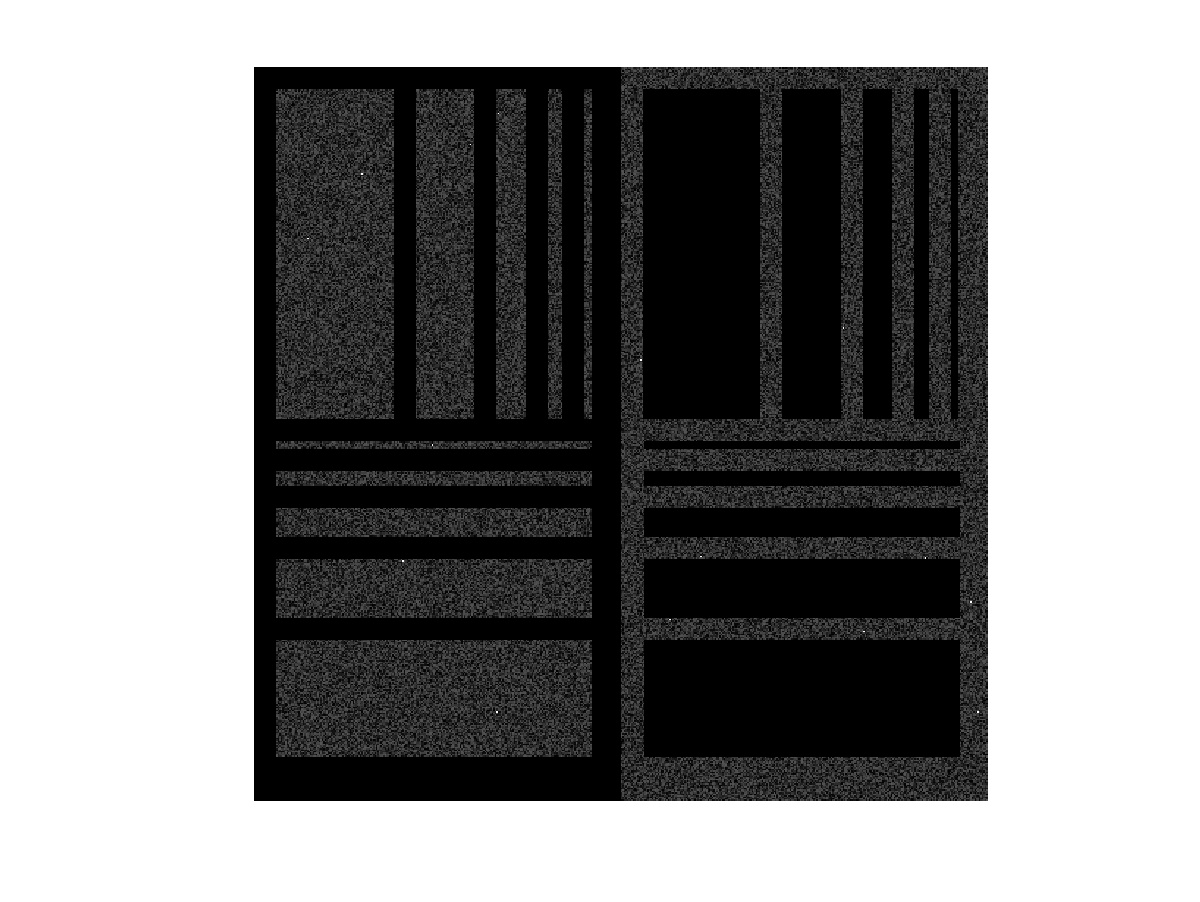
\includegraphics[width=\linewidth]{Eq_Phantom_0p000_4_1_1.jpg}
%	%\caption{Phantom $P_{1,4,0.0}$}\label{fig:awesome_image1}
%\endminipage\hfill
%\minipage{0.20\textwidth}
%  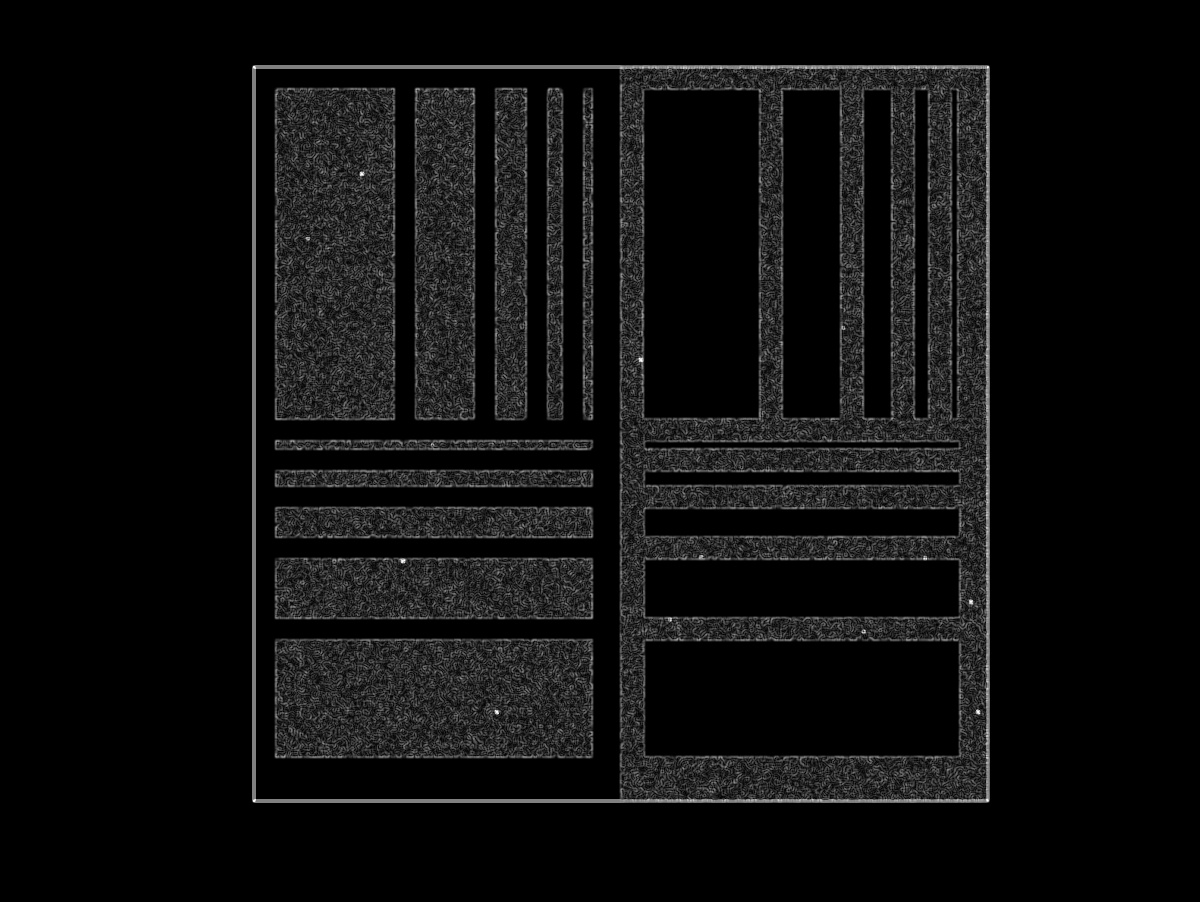
\includegraphics[width=\linewidth]{sobel_Eq_Phantom_0p000_4_1_1.jpg}
%  \caption{Sobel}\label{fig:awesome_image2}
%\endminipage\hfill
%\minipage{0.20\textwidth}%
%  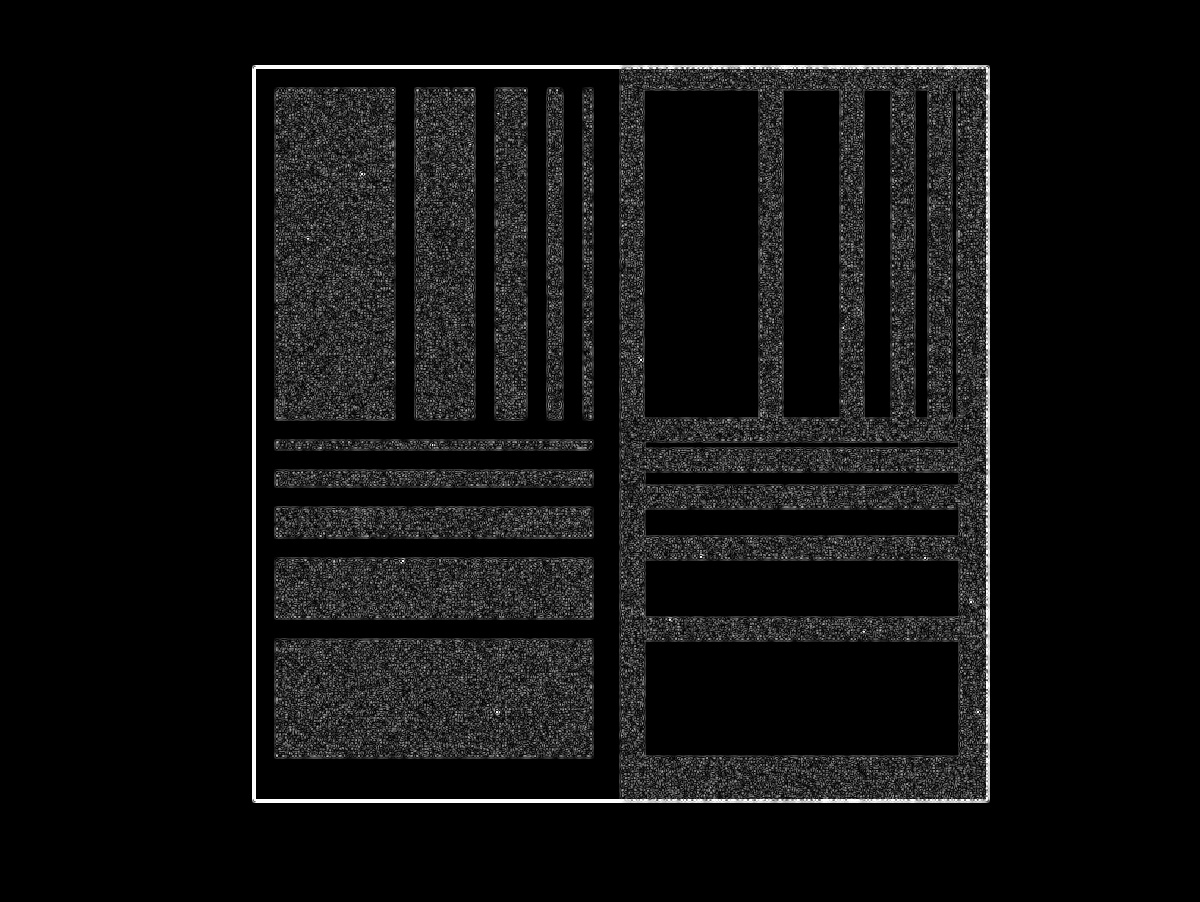
\includegraphics[width=\linewidth]{lap_Eq_Phantom_0p000_4_1_1.jpg}
%  \caption{Laplaciano}\label{fig:awesome_image3}
%\endminipage\hfill
%\minipage{0.20\textwidth}%
%  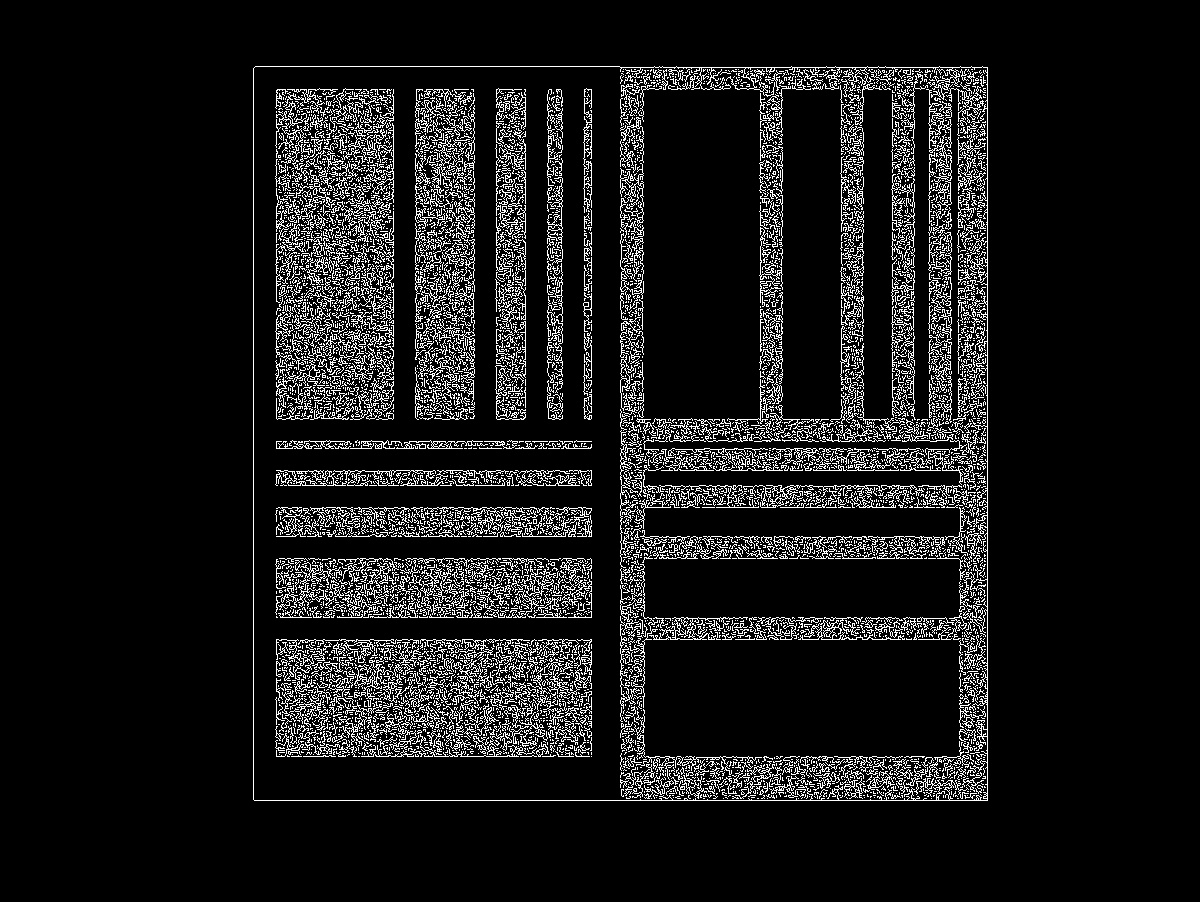
\includegraphics[width=\linewidth]{canny_Eq_Phantom_0p000_4_1_1.jpg}
%  \caption{Canny}\label{fig:awesome_image3}
%\endminipage\hfill
%\minipage{0.20\textwidth}%
%  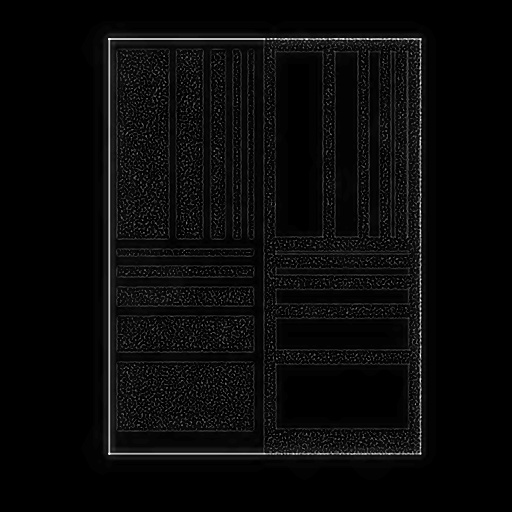
\includegraphics[width=\linewidth]{mult_Eq_Phantom_0p000_4_1_1.jpg}
%	\caption{Multigrid(Piramidal)}\label{fig:awesome_image3}
%\endminipage\hfill
%%%%% Segunda linha
%\minipage{0.20\textwidth}
%  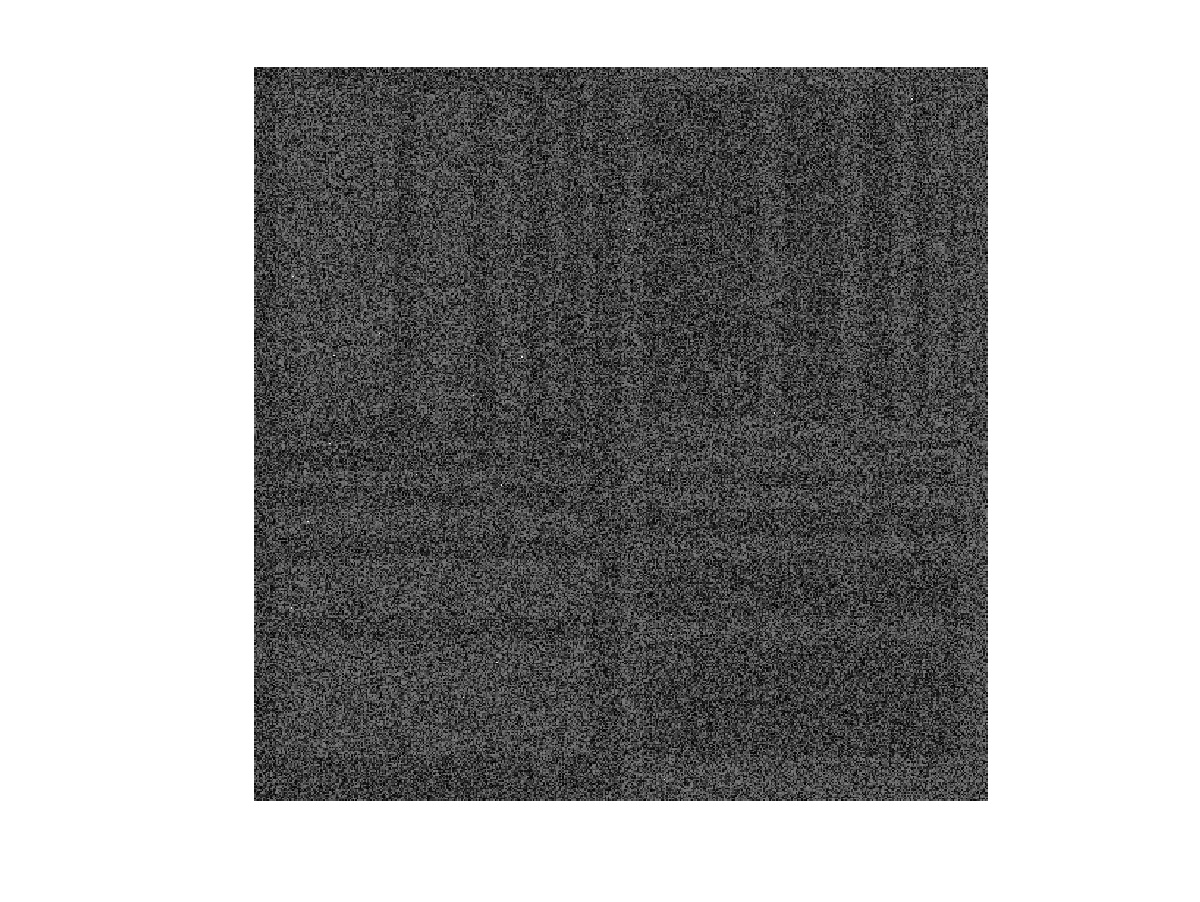
\includegraphics[width=\linewidth]{Eq_Phantom_0p500_4_1_1.jpg}
%	\caption{Phantom $P_{1,4,0.5}$}\label{fig:awesome_image1}
%\endminipage\hfill
%\minipage{0.20\textwidth}%
%  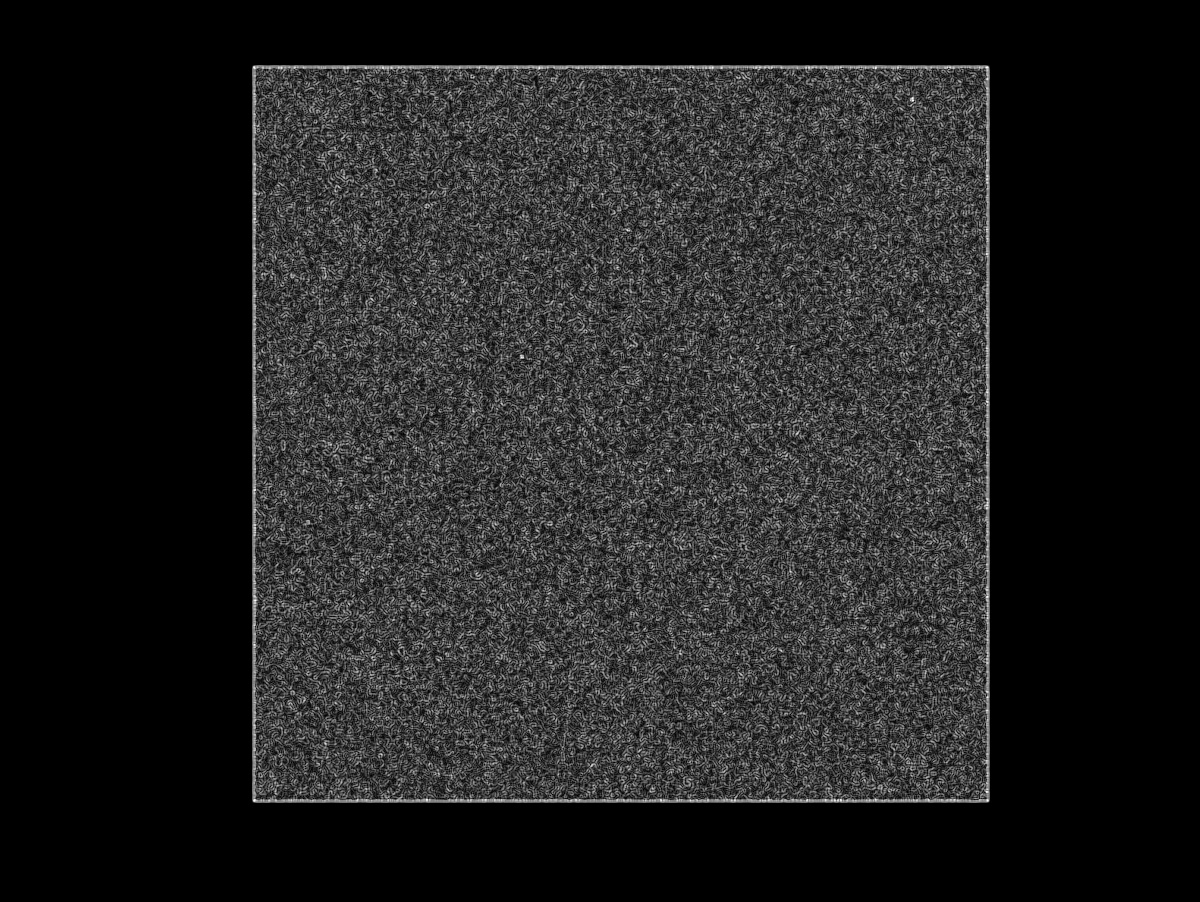
\includegraphics[width=\linewidth]{sobel_Eq_Phantom_0p500_4_1_1.jpg}
%  \caption{Sobel}\label{fig:awesome_image3}
%\endminipage\hfill
%\minipage{0.20\textwidth}%
%  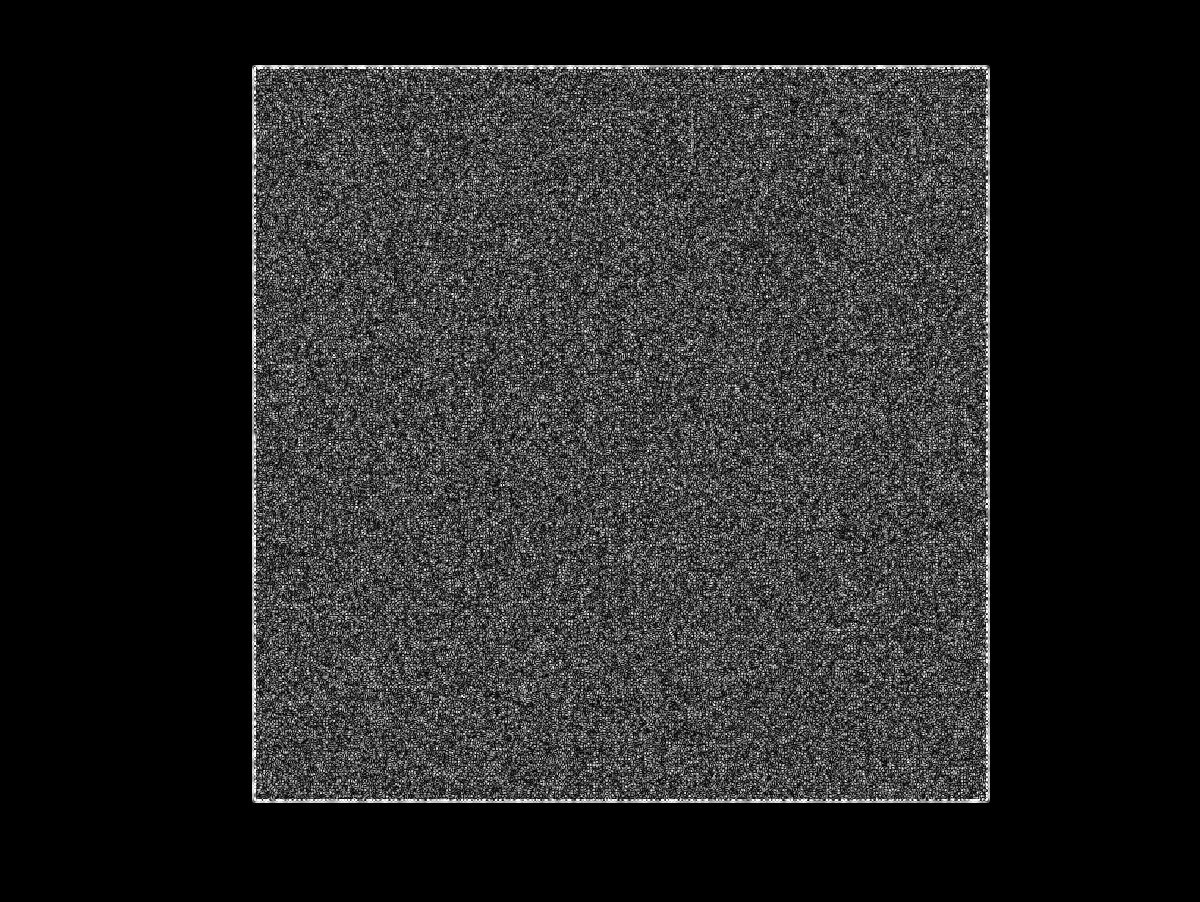
\includegraphics[width=\linewidth]{lap_Eq_Phantom_0p500_4_1_1.jpg}
%  \caption{Laplaciano}\label{fig:awesome_image3}
%\endminipage\hfill
%\minipage{0.20\textwidth}%
%  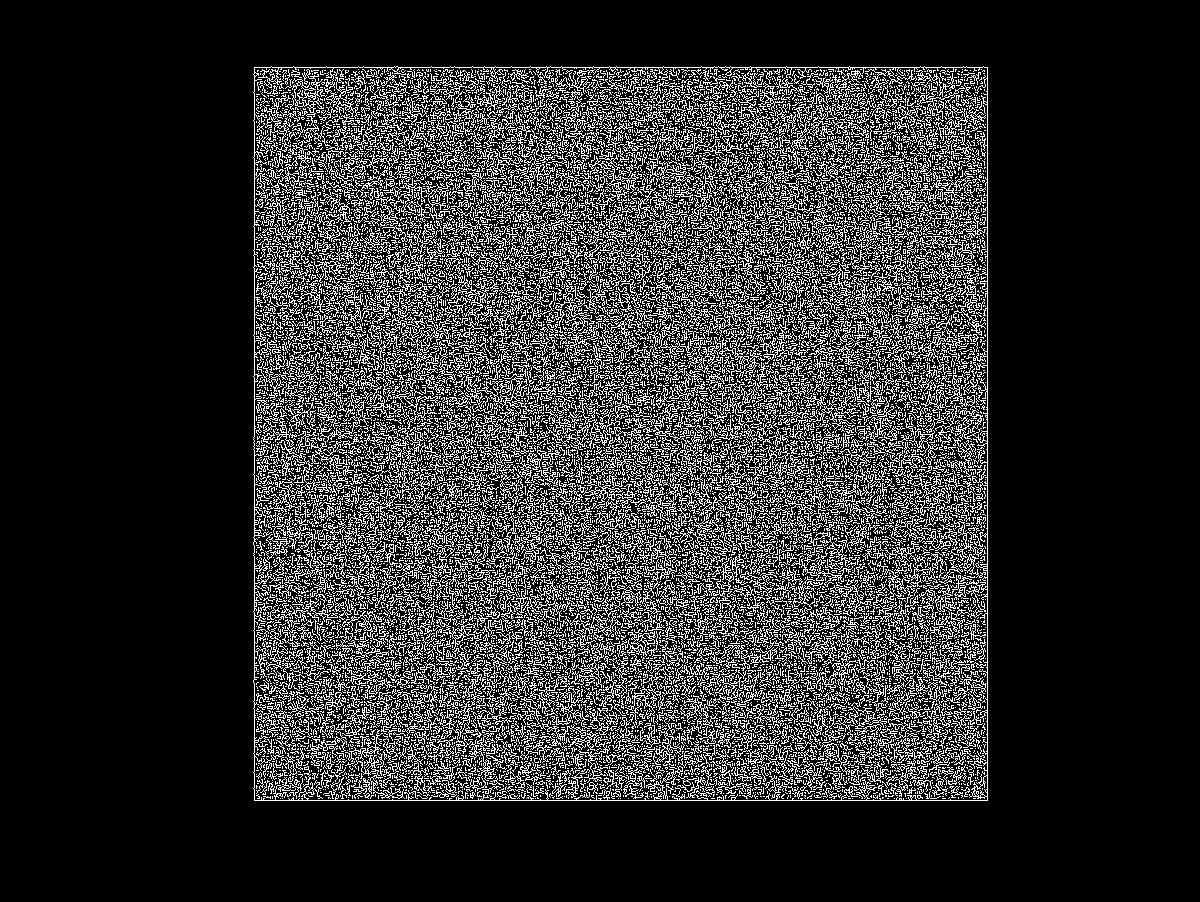
\includegraphics[width=\linewidth]{canny_Eq_Phantom_0p500_4_1_1.jpg}
%  \caption{Canny}\label{fig:awesome_image3}
%\endminipage\hfill
%\minipage{0.20\textwidth}%
%  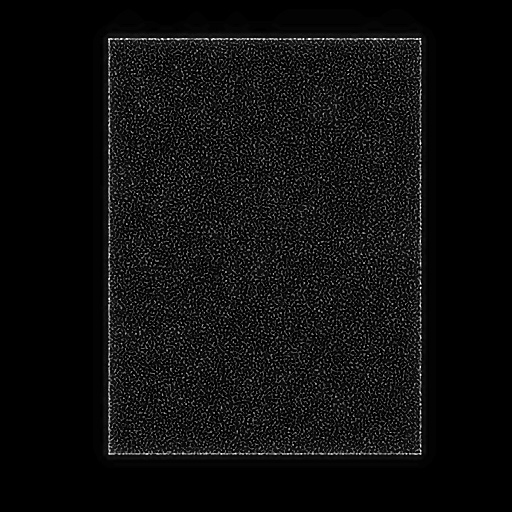
\includegraphics[width=\linewidth]{mult_Eq_Phantom_0p500_4_1_1.jpg}
%	\caption{Multigrid(Piramidal)}\label{fig:awesome_image3}
%\endminipage\hfill
%%%%% Terceira  linha
%\minipage{0.20\textwidth}
%  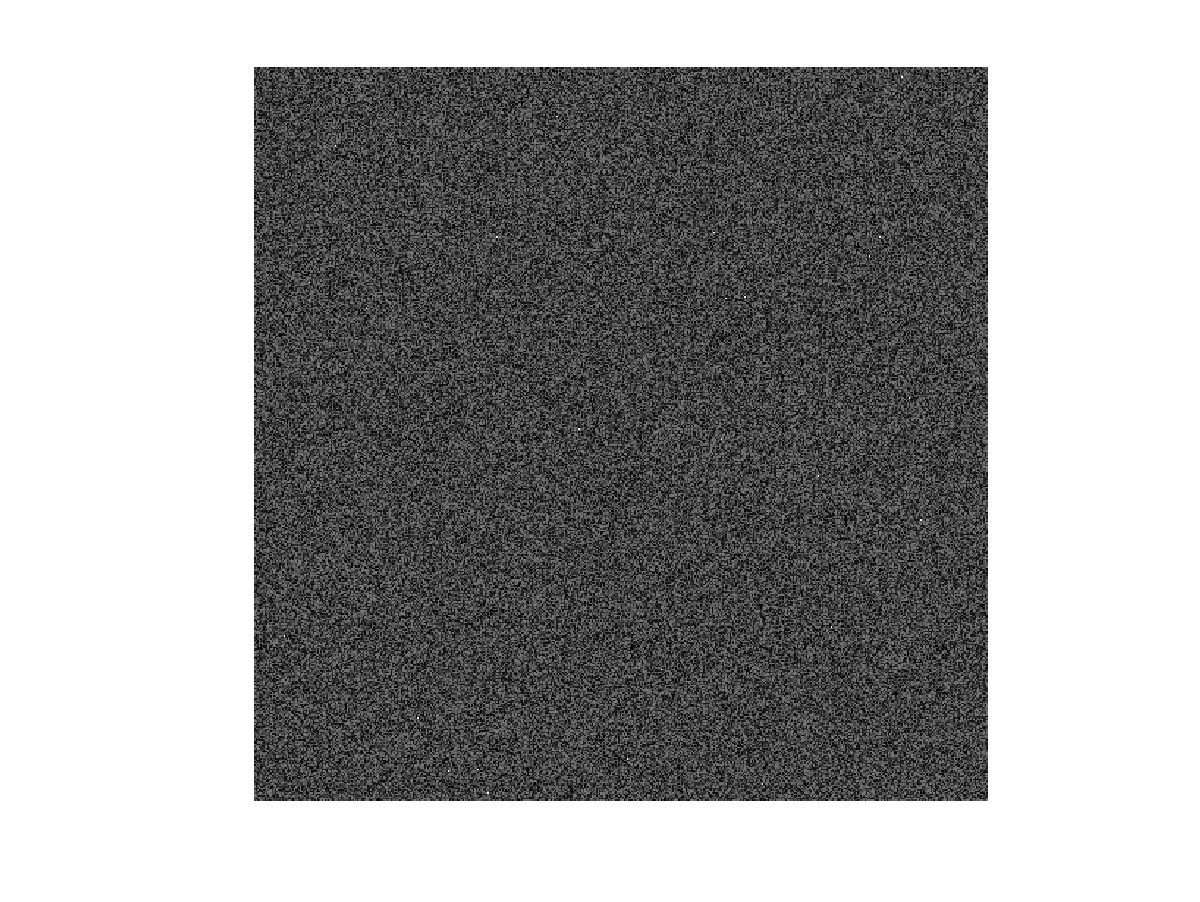
\includegraphics[width=\linewidth]{Eq_Phantom_0p700_4_1_1.jpg}
%	\caption{Phantom $P_{1,4,0.7}$}\label{fig:awesome_image1}
%\endminipage\hfill
%\minipage{0.20\textwidth}%
%  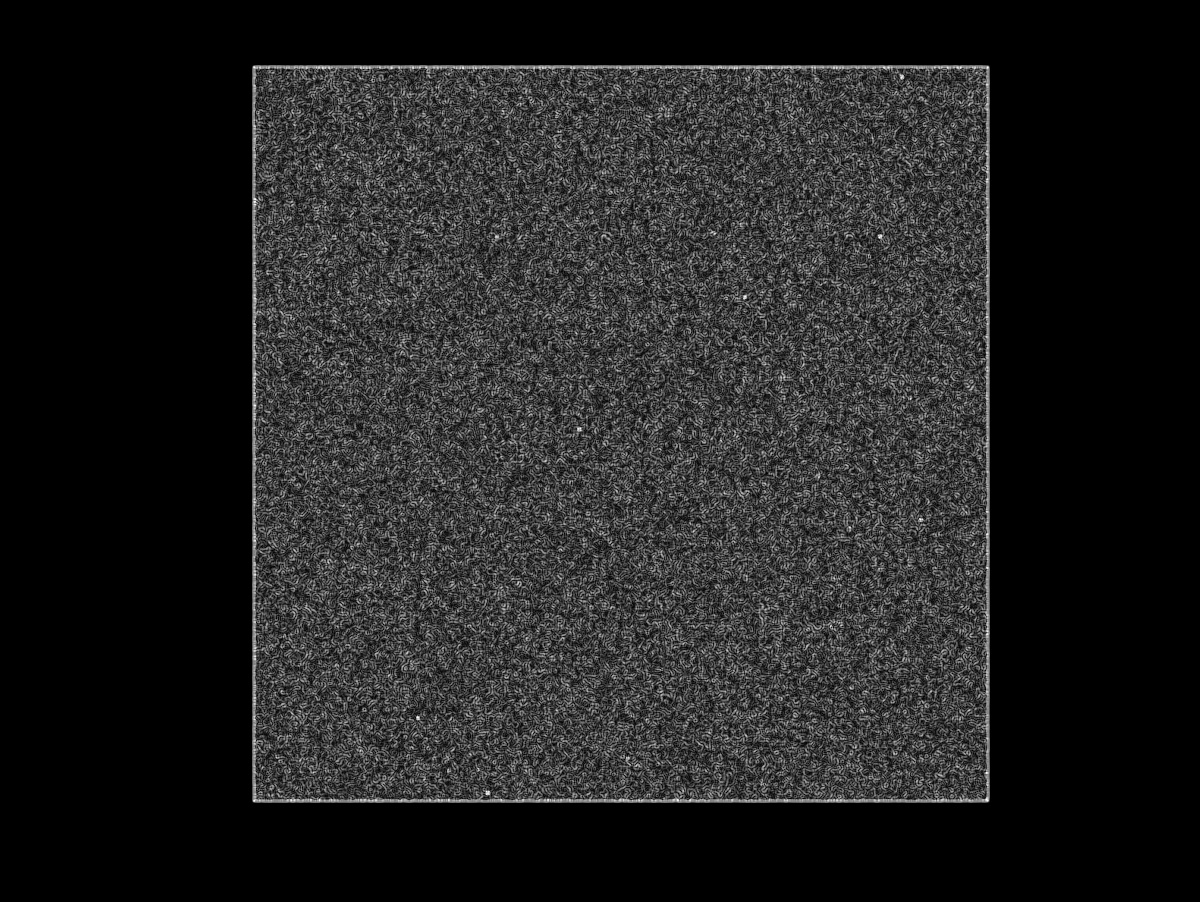
\includegraphics[width=\linewidth]{sobel_Eq_Phantom_0p700_4_1_1.jpg}
%  \caption{Sobel}\label{fig:awesome_image3}
%\endminipage\hfill
%\minipage{0.20\textwidth}%
%  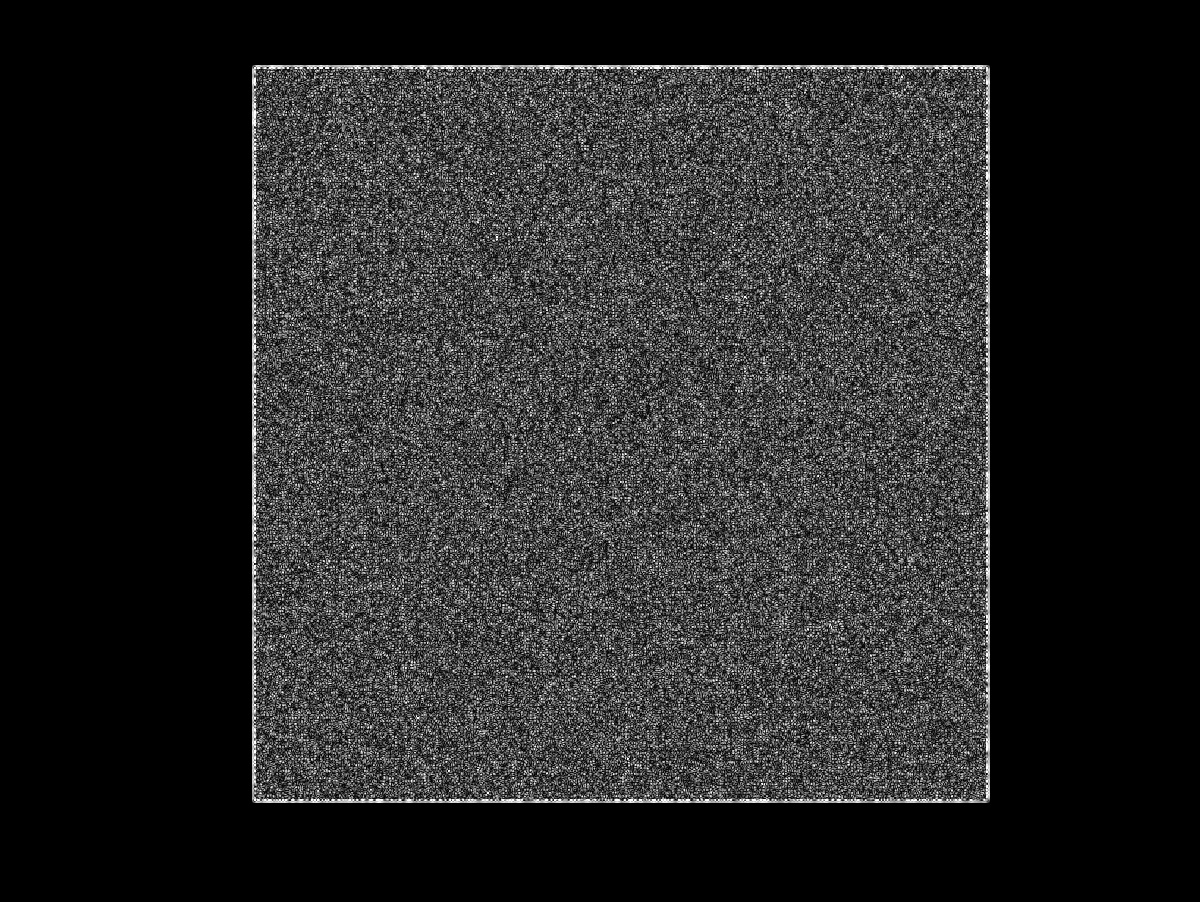
\includegraphics[width=\linewidth]{lap_Eq_Phantom_0p700_4_1_1.jpg}
%  \caption{Laplaciano}\label{fig:awesome_image3}
%\endminipage\hfill
%\minipage{0.20\textwidth}%
%  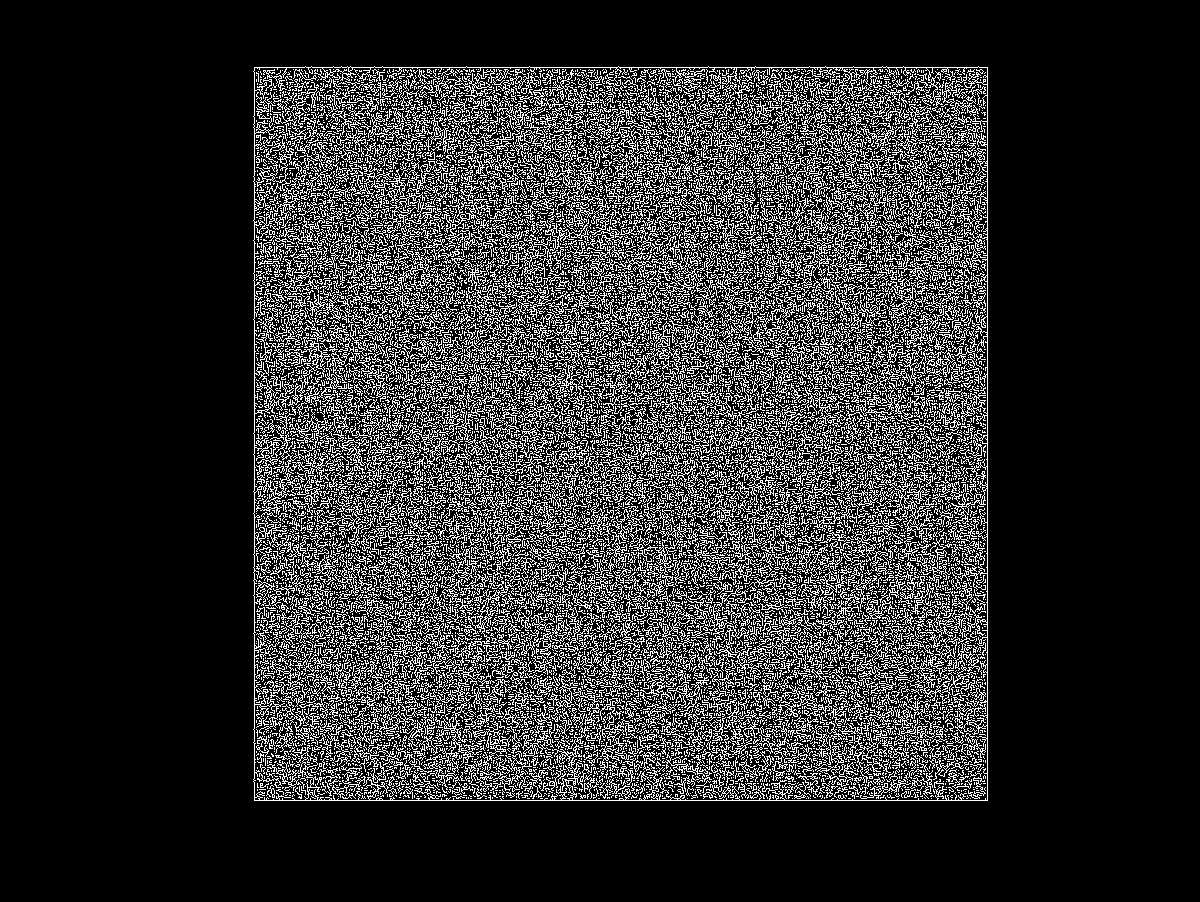
\includegraphics[width=\linewidth]{canny_Eq_Phantom_0p700_4_1_1.jpg}
%  \caption{Canny}\label{fig:awesome_image3}
%\endminipage\hfill
%\minipage{0.20\textwidth}%
%  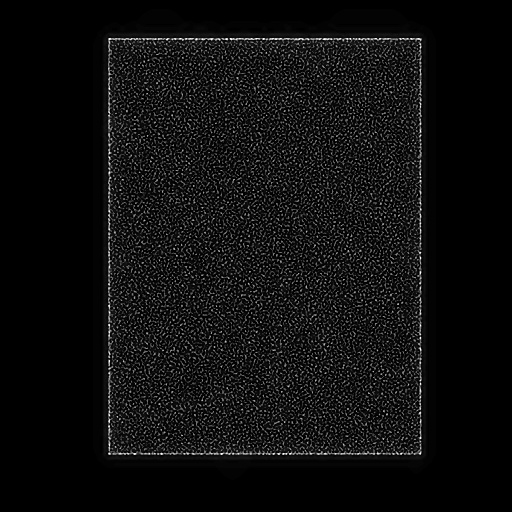
\includegraphics[width=\linewidth]{mult_Eq_Phantom_0p700_4_1_1.jpg}
%  \caption{Multigrid (Piramidal)}\label{fig:awesome_image3}
%\endminipage
%\caption{Phanton-Sobel-Laplaciano-Canny-Multgrid}\label{fig:awesome_image3}
%\end{figure}


%\begin{table}[h]
%\centering
%\caption{Tabela de tempo para os métodos propostos}.
%\begin{tabular}{|c|c|c|c|}
%\hline                  
%Método & Tempo & Taxa  & Tempo($\%$) \\
%\hline                  
%Sobel   & 0.0541s  &  $1.05tr$& $5\%$   \\
%LoG     & 0.0513s  &  $tr$& $*$   \\
%Log Pir & 0.0600s  &  $1.16tr$& $16\%$ \\
%OLM     & 0.0622s  &  $1.21tr$& $21\%$ \\
%OLMM    & 0.0564s  &  $1.09tr$& $9\%$    \\ 
%\hline                  
%\end{tabular}
%\end{table}


%\begin{figure}[!htb]
%\centering
%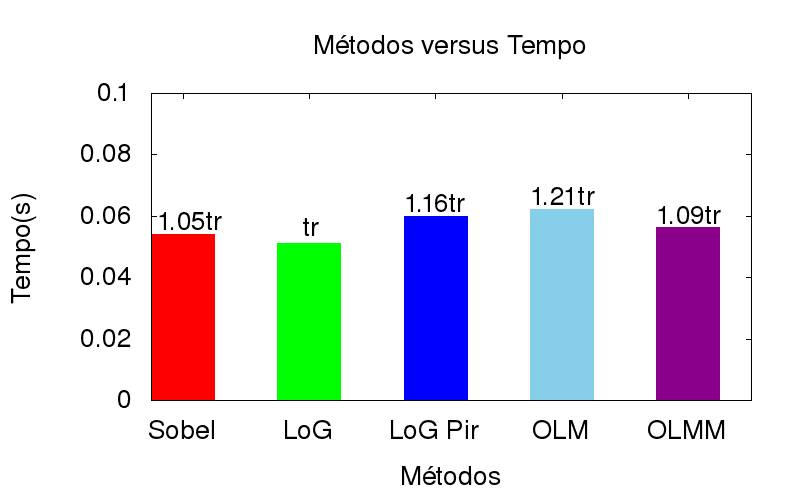
\includegraphics[width=3.0in]{output.jpg}
%\label{output}
%\caption{Gráfico Métodos versus Tempo.}
%\end{figure}


\section{Conclusão}

\bibliographystyle{unsrt}
\bibliography{../bibliografia}
\end{document}
